\chapter{Existence de l'Équilibre de Nash}

\section{Non-existence de l'Équilibre de Nash}

L'existence d'un équilibre de Nash n'est pas garantie. Plusieurs obstacles peuvent l'empêcher.

\subsection{Exemples de Non-existence}
\begin{enumerate}
    \item \textbf{Absence de compacité :} 2 joueurs sur $[0, +\infty[$, $u_1 = x_1$, $u_2 = x_2$. Pas d'équilibre car les gains ne sont pas bornés (chacun veut jouer $+\infty$).
    \item \textbf{Absence de convexité ou continuité (Matching Pennies continu) :}
    C'est le jeu "I like you, you don't like me". $u_1(x_1, x_2) = -|x_1 - x_2|$ (veut se rapprocher) et $u_2(x_1, x_2) = |x_1 - x_2|$ (veut s'éloigner) sur $[0,1]$.
    \begin{itemize}
        \item Si $x_1 = x_2$, P2 veut s'éloigner (jouer $0$ ou $1$).
        \item Si $x_1 \ne x_2$, P1 veut se rapprocher de $x_2$.
        \item Il n'y a aucun point fixe, donc aucun équilibre en stratégies pures.
    \end{itemize}
    
\begin{center}
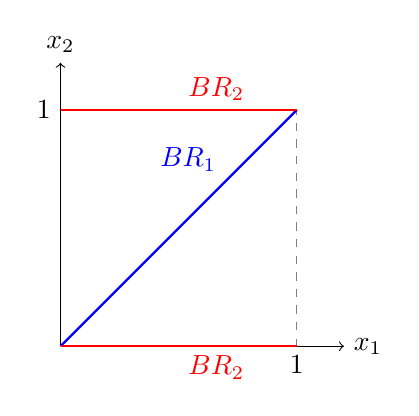
\begin{tikzpicture}[scale=3]
    % Axes
    \draw[->] (0,0) -- (1.2,0) node[right] {$x_1$};
    \draw[->] (0,0) -- (0,1.2) node[above] {$x_2$};
    % Unit square
    \draw[gray, dashed] (0,1) -- (1,1) -- (1,0);
    \node[below] at (1,0) {1};
    \node[left] at (0,1) {1};
    % BR1: x_1 = x_2 (diagonal)
    \draw[thick, blue] (0,0) -- (1,1);
    \node[blue, above left] at (0.7,0.7) {$BR_1$};
    % BR2: x_2 = 0 or x_2 = 1 (boundaries)
    \draw[thick, red] (0,0) -- (1,0);
    \draw[thick, red] (0,1) -- (1,1);
    \node[red, below right] at (0.5,0) {$BR_2$};
    \node[red, above right] at (0.5,1) {$BR_2$};
\end{tikzpicture}
\captionof{figure}{Matching Pennies Continu : les meilleures réponses ne se croisent jamais.}
\end{center}
\begin{figureexplanation}
Dans ce jeu à somme nulle continu sur le carré (Matching Pennies), les meilleures réponses (lignes bleue et rouge) ne se croisent jamais. Il n'y a donc pas d'intersection des graphes de meilleure réponse, ce qui implique qu'il n'existe pas d'équilibre de Nash en stratégies pures.
\end{figureexplanation}

\end{enumerate}

\begin{remarque}[Illustration Culturelle]
Le Professeur associe souvent cette frustration de la non-existence au tableau \textbf{"Le Cri" d'Edvard Munch} : l'angoisse de ne pas trouver de solution stable dans un monde sans convexité ni compacité.
\end{remarque}

\subsection{Obstacles à l'existence}
Les principaux obstacles à l'existence d'un équilibre de Nash sont :
\begin{itemize}
    \item \textbf{Ensembles d'actions non convexes :} Dans les jeux finis, les ensembles de stratégies présentent des "trous".
    \item \textbf{Ensembles d'actions non bornés ou non fermés : } Problème de compacité.
    \item \textbf{Fonctions de gain discontinues.}
    \item \textbf{Absence de quasi-concavité :} Si la fonction de gain n'est pas quasi-concave, l'ensemble des meilleures réponses peut ne pas être convexe.
\end{itemize}

\section{Quasiconcavité et Goût pour le Risque}

La quasi-concavité est une propriété cruciale pour l'existence. Elle est intimement liée à la notion d'aversion ou de goût pour le risque.

\begin{definition}[Quasiconcavité]
Soit $X$ un ensemble convexe. $f: X \rightarrow \mathbb{R}$ est \textbf{quasiconcave} si pour tout $\lambda \in [0,1]$ et tout $(x, y) \in X^2$ :
$$f(\lambda x + (1-\lambda)y) \ge \min\{f(x), f(y)\}$$
\textbf{Caractérisation équivalente :} $f$ est quasiconcave si et seulement si tous ses \textbf{ensembles de niveau supérieur} sont convexes :
$$\forall \alpha \in \mathbb{R}, \quad S_{\alpha}(f) = \{x \in X : f(x) \ge \alpha\} \text{ est convexe.}$$
\end{definition}

\begin{exemple}[Intuition Économique : Goût pour le risque]
Considérons $u(x) = x^2$ sur $\mathbb{R}$.
\begin{itemize}
    \item Cette fonction est convexe (parabole).
    \item Elle n'est \textbf{pas quasiconcave} sur $\mathbb{R}$ (ex: $S_1(f) = ]-\infty, -1] \cup [1, +\infty[$ n'est pas convexe).
    \item \textbf{Interprétation :} Un agent avec une telle utilité est "Risk-Loving" (aimant le risque). Il préfère un résultat incertain (ex: une loterie entre -2 et 2, moyenne 0) à son équivalent certain (0), car $u(0)=0 < 0.5 u(-2) + 0.5 u(2) = 4$.
\end{itemize}

\begin{center}
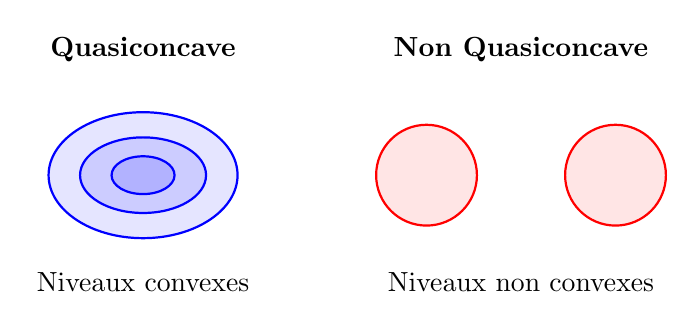
\begin{tikzpicture}[scale=0.8]
    % Quasiconcave (left)
    \node at (2, 3.5) {\textbf{Quasiconcave}};
    \draw[thick, blue, fill=blue!10] (2,1.5) ellipse (1.5 and 1);
    \draw[thick, blue, fill=blue!20] (2,1.5) ellipse (1 and 0.6);
    \draw[thick, blue, fill=blue!30] (2,1.5) ellipse (0.5 and 0.3);
    \node at (2, -0.2) {Niveaux convexes};
    
    % Not quasiconcave (right)
    \node at (8, 3.5) {\textbf{Non Quasiconcave}};
    \draw[thick, red, fill=red!10] (6.5,1.5) ellipse (0.8 and 0.8);
    \draw[thick, red, fill=red!10] (9.5,1.5) ellipse (0.8 and 0.8);
    \node at (8, -0.2) {Niveaux non convexes};
\end{tikzpicture}
\captionof{figure}{Niveaux supérieurs : convexes (quasiconcave) vs non convexes.}
\end{center}
\begin{figureexplanation}
La quasi-concavité est caractérisée par la convexité des ensembles de niveau supérieur $S_\alpha = \{x \mid f(x) \ge \alpha\}$.
\begin{itemize}
    \item À gauche : $S_\alpha$ (zones colorées) est toujours convexe. La fonction est quasi-concave.
    \item À droite : Pour certains $\alpha$, $S_\alpha$ est disjoint (union de deux ensembles séparés), donc non convexe. La fonction n'est pas quasi-concave.
\end{itemize}
\end{figureexplanation}

\end{exemple}

\section{Théorème de Glicksberg}
C'est le théorème fondamental assurant l'existence d'un équilibre de Nash en stratégies pures.

\begin{theoreme}[Glicksberg]
Soit un jeu $G = (N, (X_i)_{i \in N}, (u_i)_{i \in N})$ tel que :
\begin{enumerate}
    \item $X_i$ est un sous-ensemble \textbf{compact et convexe} d'un espace vectoriel topologique.
    \item $u_i$ est \textbf{continue} sur $X = \prod X_i$.
    \item $x_i \mapsto u_i(x_i, x_{-i})$ est \textbf{quasiconcave} pour tout $x_{-i}$.
\end{enumerate}
Alors, il existe un équilibre de Nash.
\end{theoreme}

\subsection{Démonstration (Rigueur Examen)}
La preuve repose sur l'application du théorème de point fixe à la correspondance de meilleure réponse $B(x) = \prod B_i(x_{-i})$.

\paragraph{Pourquoi Kakutani et pas Brouwer ?}
Le Théorème de Brouwer s'applique aux \textbf{fonctions} continues. Ici, la meilleure réponse n'est pas unique (c'est un ensemble), c'est une \textbf{correspondance}. On doit donc utiliser le \textbf{Théorème de Kakutani}.

\begin{center}
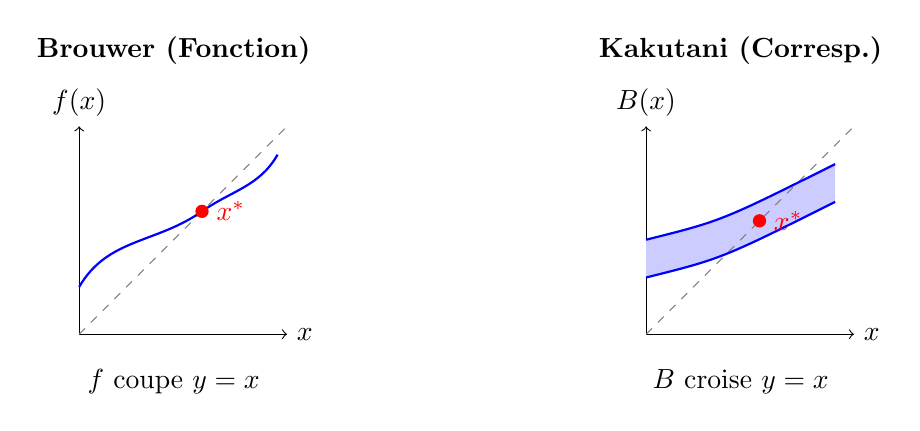
\begin{tikzpicture}[scale=1.2]
    % Brouwer (left)
    \begin{scope}[shift={(-3.5,0)}]
        \node at (1, 3.0) {\textbf{Brouwer (Fonction)}};
        \draw[->] (0,0) -- (2.2,0) node[right] {$x$};
        \draw[->] (0,0) -- (0,2.2) node[above] {$f(x)$};
        \draw[gray, dashed] (0,0) -- (2.2,2.2);
        
        % Curve adjusted to cross exactly at (1.3, 1.3)
        \draw[thick, blue] (0,0.5) to[out=60, in=215] (1.3,1.3) to[out=35, in=240] (2.1,1.9);
        
        \fill[red] (1.3,1.3) circle (2pt);
        \node[red, right] at (1.35,1.3) {$x^*$};
        \node at (1,-0.5) {$f$ coupe $y=x$};
    \end{scope}
    
    % Kakutani (right)
    \begin{scope}[shift={(2.5,0)}]
        \node at (1, 3.0) {\textbf{Kakutani (Corresp.)}};
        \draw[->] (0,0) -- (2.2,0) node[right] {$x$};
        \draw[->] (0,0) -- (0,2.2) node[above] {$B(x)$};
        
        % Correspondence as a convex-valued band
        % Adjusted to cross the diagonal more sharply
        % Starts clearly above diagonal, ends clearly below
        \fill[blue!20] (0,0.6) .. controls (0.8,0.8) .. (2,1.4) 
            -- (2,1.8) .. controls (0.8,1.2) .. (0,1.0) -- cycle;
            
        % Dashed line (diagonal) - DRAWN AFTER FILL for visibility
        \draw[gray, dashed] (0,0) -- (2.2,2.2);

        % Border lines of the correspondence
        \draw[thick, blue] (0,0.6) .. controls (0.8,0.8) .. (2,1.4);
        \draw[thick, blue] (0,1.0) .. controls (0.8,1.2) .. (2,1.8);
        
        % Fixed point intersection
        % Intersection is roughly at (1.2, 1.2) which is inside the band
        % At x=1.2:
        % Lower ~ 0.6 + (0.8)*0.6 = 1.08? No bezier math is distinct
        % Visually (1.2, 1.2) works well with these control points
        \fill[red] (1.2,1.2) circle (2pt);
        \node[red, right] at (1.25,1.2) {$x^*$};
        
        \node at (1,-0.5) {$B$ croise $y=x$};
    \end{scope}
\end{tikzpicture}
\captionof{figure}{Brouwer vs Kakutani : fonction vs correspondance.}
\end{center}
\begin{figureexplanation}
\textbf{Comparaison des théorèmes :}
\begin{itemize}
    \item \textbf{Brouwer (Gauche) :} Si $f$ est une \textit{fonction} continue de $[0,1]$ dans lui-même, son graphe (courbe bleue) doit nécessairement croiser la diagonale (pointillés). L'intersection est un point fixe $x^* = f(x^*)$.
    \item \textbf{Kakutani (Droite) :} Si $B$ est une \textit{correspondance} (ensemble de valeurs) à graphe fermé et valeurs convexes (la zone bleue est "pleine" verticalement), son graphe doit aussi croiser la diagonale. L'intersection $x^*$ vérifie $x^* \in B(x^*)$, c'est un point fixe.
\end{itemize}
\end{figureexplanation}

\paragraph{Vérification des 3 conditions de Kakutani :}
Pour appliquer Kakutani à $B : X \rightrightarrows X$, il faut vérifier :
\begin{enumerate}
    \item \textbf{Non-vacuité (Non-empty) :} Comme $u_i$ est continue sur un ensemble compact $X_i$, elle atteint son maximum (Théorème de Weierstrass). Donc $B_i(x_{-i}) \ne \emptyset$.
    \item \textbf{Convexe (Convex values) :} Comme $u_i$ est quasi-concave par rapport à $x_i$, l'ensemble des maximisateurs $B_i(x_{-i})$ est convexe.
    \item \textbf{Graphe fermé (Closed Graph) :} C'est une conséquence de la continuité globale de $u_i$ (Théorème du Maximum de Berge). Si une suite $x^n \to x$ et $y^n \in B(x^n)$ avec $y^n \to y$, alors $y \in B(x)$.
\end{enumerate}
Toutes les conditions étant réunies, $B$ admet un point fixe $x^* \in B(x^*)$, qui est un équilibre de Nash.

\section{Exemples Résolus}

\subsection{Public Good Provision}
Pour $n$ habitants, $u_i = W - x_i + \sqrt{\sum x_j}$. On cherche un équilibre symétrique $(a, \dots, a)$.
Posons $f(x_i) = W - x_i + \sqrt{(n-1)a + x_i}$. La condition du premier ordre $f'(a) = 0$ donne :
$$-1 + \frac{1}{2\sqrt{na}} = 0 \iff 2\sqrt{na} = 1 \iff 4na = 1 \iff a = \frac{1}{4n}$$

\subsection{Rent-seeking (Tullock)}
$n$ firmes, payoff $u_i = \frac{x_i}{\sum x_j}V - cx_i$. Pour un équilibre symétrique $a$ :
$$f'(x_i) = \frac{V((n-1)a + x_i) - Vx_i}{((n-1)a + x_i)^2} - c = 0$$
En $x_i = a$, on obtient $\frac{(n-1)V}{n^2 a} = c$, d'où $a = \frac{n-1}{cn^2}V$.

\section{Extensions et Cas Limites (Pour aller plus loin)}

\begin{itemize}
    \item \textbf{Argument de Coercivité :} Si les ensembles d'actions ne sont pas compacts (ex: $X_i = \mathbb{R}$), l'équilibre peut quand même exister si les fonctions sont \textbf{coercives}, c'est-à-dire si $\lim_{|x_i| \to \infty} u_i(x) = -\infty$. Cela permet de restreindre l'analyse à un sous-ensemble compact suffisamment grand.
\end{itemize}

\begin{exemple}[Exam 2023 : Preuve de Coercivité]
\textbf{Question :}
Prouvez l'existence d'un équilibre de Nash pour un jeu où les fonctions d'utilité sont coercives.

\textbf{Correction :}
\begin{enumerate}
    \item Par hypothèse, $\lim_{|x| \to \infty} u_i(x, y) = -\infty$. La fonction est donc coercive sur un ensemble fermé, ce qui garantit l'existence d'un maximum et donc d'une meilleure réponse.
    \item En considérant une séquence de jeux sur des ensembles compacts $X_n \times Y_n$, on applique le théorème de Glicksberg pour garantir l'existence d'un équilibre de Nash $(\bar{x}_n, \bar{y}_n)$.
    \item Puisque les meilleures réponses sont bornées par coercivité, la séquence converge vers un équilibre $(\bar{x}, \bar{y})$ du jeu original.
\end{enumerate}
\end{exemple}

\subsection{Remarques sur l'existence (Hors programme examen)}
Dans de nombreux modèles économiques, les fonctions de gain sont discontinues. L'existence d'un équilibre de Nash peut tout de même être garantie sous certaines conditions :
\begin{itemize}
    \item \textbf{Reny (1999)} : Concept de "better-reply security".
    \item \textbf{Bich-Laraki (2017)} : Travaux sur les jeux avec payoffs discontinus.
    \item \textbf{Bich (2004)} : Version non-continue du théorème de point fixe de Brouwer.
\end{itemize}

\paragraph{Jeu de Consensus}
Trois joueurs $i \in \{1,2,3\}$, $X_i = [0,1]$.
\[ u_1(x_1, x_2, x_3) = - \left| x_1 - \frac{x_2 + x_3}{2} \right|^2 \]
Chaque joueur cherche à être le plus proche possible de la moyenne des autres.
L'équilibre est $(1/2, 1/2, 1/2)$ si l'on cherche un point fixe.

\begin{exercice}[Équilibre de Nash Symétrique]
Soit un jeu symétrique $G = (X, X, u, u)$ où $X$ est compact convexe et $u$ est continue et quasi-concave par rapport à sa première variable. Prouver à l'aide du théorème de Kakutani appliqué à la correspondance de meilleure réponse $BR$ qu'il existe un équilibre symétrique $(x^*, x^*)$.
\paragraph{Correction :}
1. Soit $BR : X \rightrightarrows X$ la correspondance de meilleure réponse du joueur type.
2. Définissons la fonction $\phi : X \to \mathcal{P}(X)$ par $\phi(x) = BR(x, x, \dots, x)$.
   
   \textbf{Méthode plus simple :}
   Soit la correspondance "réaction best-reply symétrique" $F: X \rightrightarrows X$ définie par :
   $$ y \in F(x) \iff y \in \arg\max_{z \in X} u(z, x, \dots, x) $$
   ( $y$ est la meilleure réponse d'un joueur si TOUS les autres jouent $x$).
   
   \begin{itemize}
       \item $X$ est compact convexe non vide.
       \item $F(x)$ est non vide (continuité sur compact) et convexe (quasi-concavité).
       \item $F$ a un graphe fermé (Théorème du Maximum).
   \end{itemize}
   D'après le Théorème de Kakutani, $F$ admet un point fixe $x^* \in F(x^*)$.
   Cela signifie que si tous les autres jouent $x^*$, la meilleure réponse pour moi est aussi de jouer $x^*$.
   Comme le jeu est symétrique, $(x^*, \dots, x^*)$ est un équilibre de Nash.
\end{exercice}

\section{Conclusion et Transition}
Nous avons vu que l'existence d'un équilibre de Nash en stratégies pures nécessite des conditions fortes (convexité, continuité, quasi-concavité). Lorsque ces conditions ne sont pas remplies (par exemple, dans les jeux finis où les ensembles d'actions discrets ne sont pas convexes), l'équilibre en stratégies pures peut ne pas exister (ex: Matching Pennies, Pierre-Papier-Ciseaux).

Pour garantir l'existence d'une solution stable dans tous les jeux finis, nous devons étendre notre concept de stratégie et autoriser les joueurs à randomiser leurs choix. C'est l'objet du prochain chapitre sur les \textbf{stratégies mixtes}.
